\documentclass{article}
\usepackage{geometry}
 \geometry{
 a4paper,
 total={210mm,297mm},
 left=20mm,
 right=20mm,
 top=20mm,
 bottom=20mm,
 }

\usepackage{siunitx} % Provides the \SI{}{} command for typesetting SI units
\usepackage{listings}
\usepackage{graphicx} % Required for the inclusion of images
\usepackage{enumerate}
\usepackage{float}
\usepackage{fancyvrb}
\usepackage[utf8]{inputenc}
\usepackage{listings}
\usepackage{inconsolata}

\lstset{
    frame=single,
    basicstyle=\small\ttfamily,
    language=bash
}

\setlength\parindent{0pt} % Removes all indentation from paragraphs

\title{Network Security \\ 389.159 - SS 2018 \\ Lab Exercise 3 \& Lab Exercise 4} % Title

\author{
    TEAM 02 \\
    Corentin \textsc{Bergès} (11741629) (066 506) \\
    Christoph \textsc{Echtinger-Sieghart} (00304130) (066 938)
}

\date{\today} % Date for the report
\begin{document}

\maketitle % Insert the title, author and date
\renewcommand{\arraystretch}{2} %Stretch rows

\section{Lab Exercise 3}

\subsection{rep-10}

\begin{figure}[h]
    \centering
    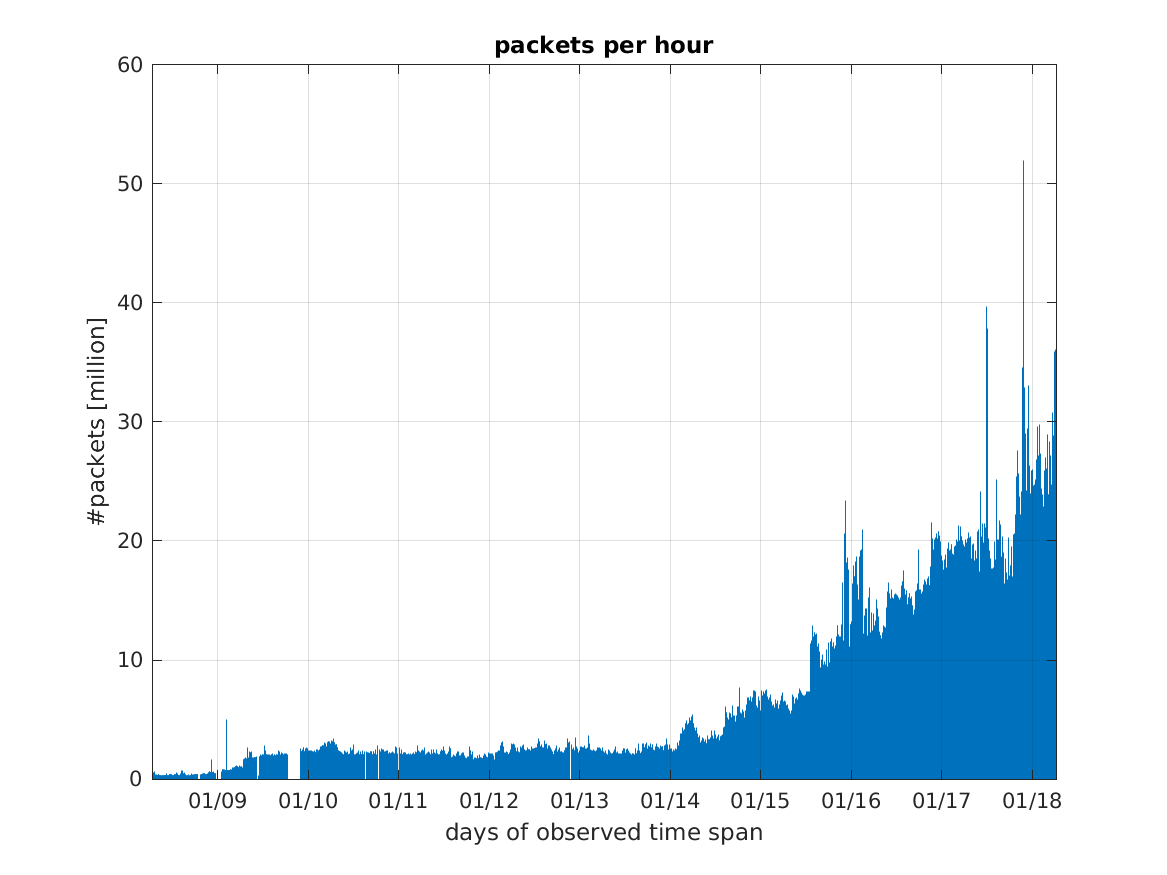
\includegraphics[scale=.8]{../exercise-3/plots/rep_10_1}
\end{figure}

\begin{figure}[h]
    \centering
    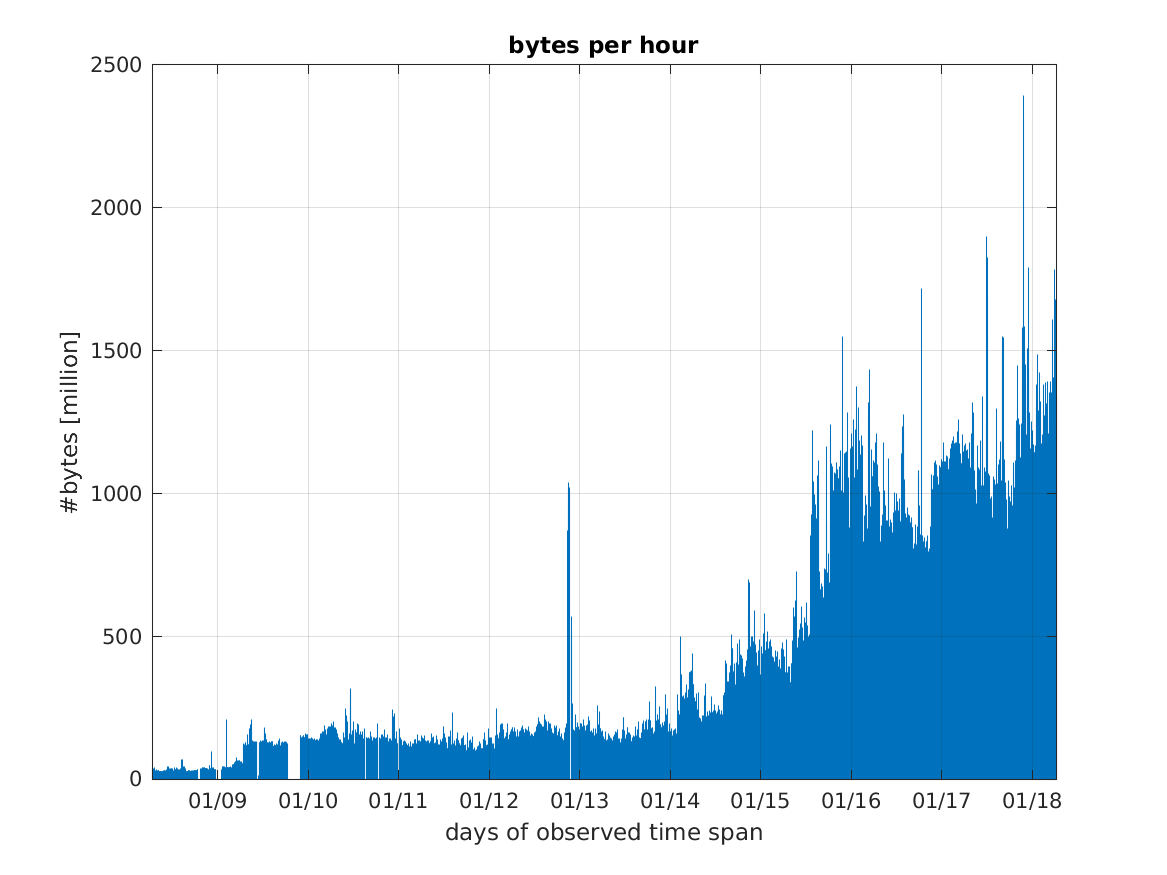
\includegraphics[scale=.8]{../exercise-3/plots/rep_10_2}
\end{figure}

\begin{figure}[h]
    \centering
    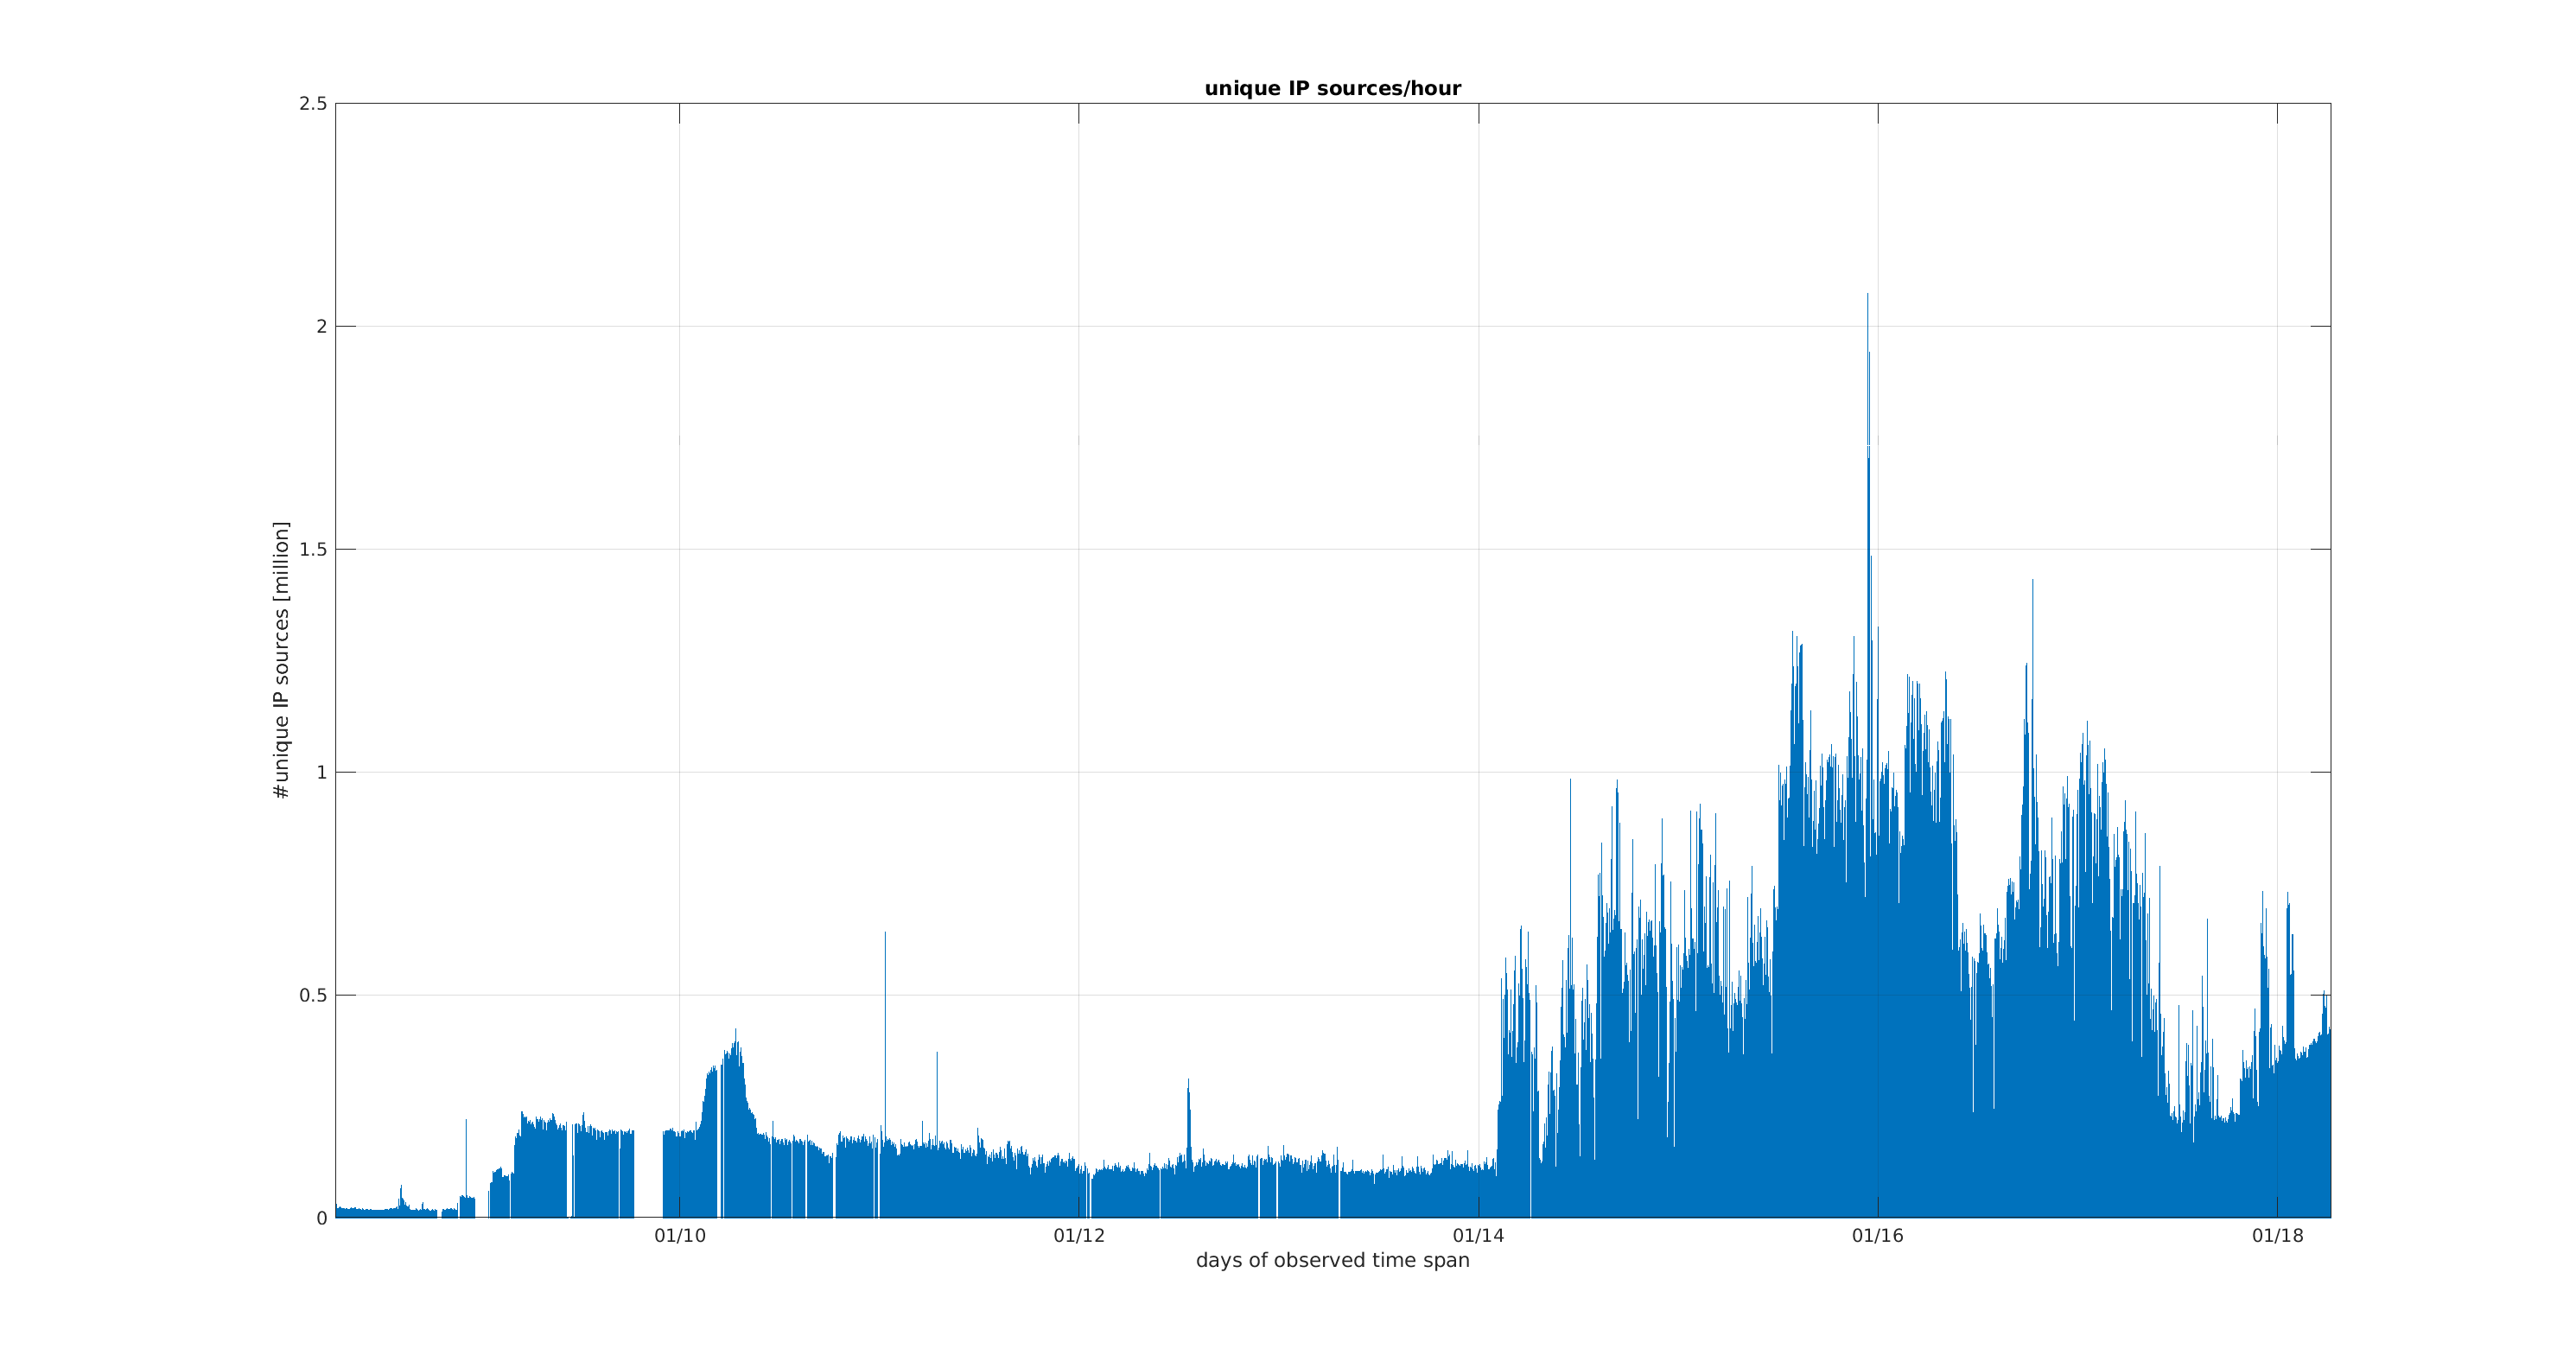
\includegraphics[scale=.8]{../exercise-3/plots/rep_10_3}
\end{figure}

\begin{figure}[h]
    \centering
    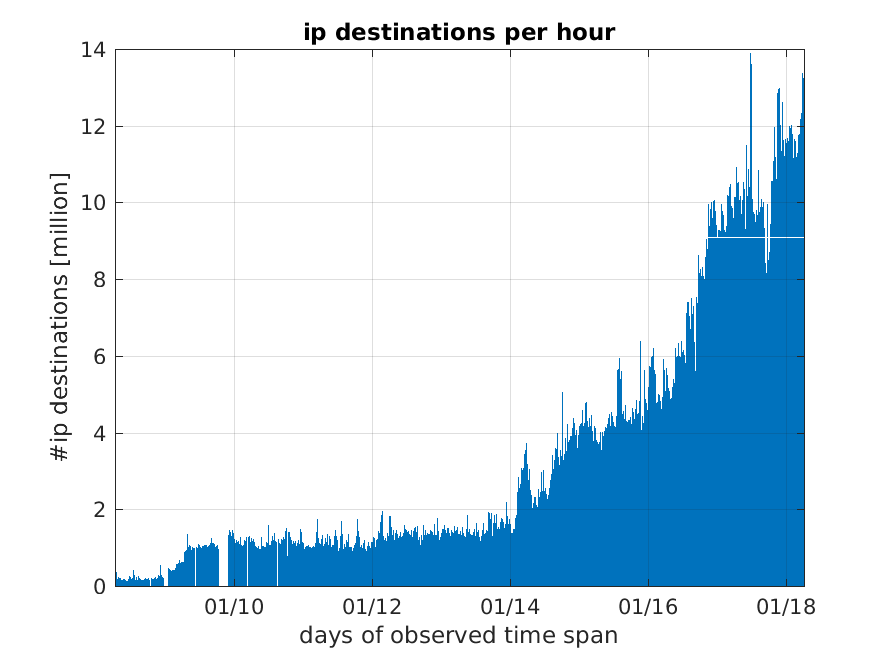
\includegraphics[scale=.8]{../exercise-3/plots/rep_10_4}
\end{figure}

\begin{figure}[h]
    \centering
    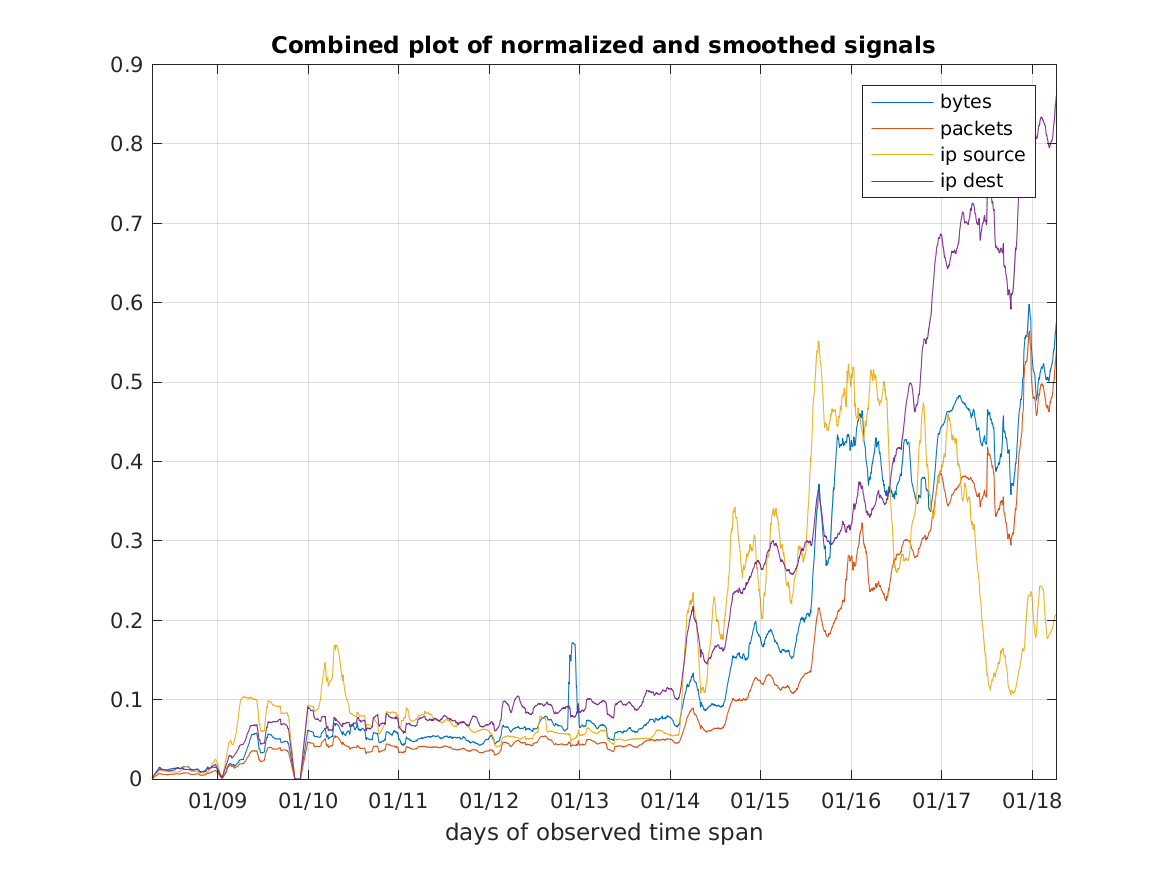
\includegraphics[scale=.8]{../exercise-3/plots/rep_10_optional}
\end{figure}

\subsection{rep-11}



\subsection{rep-12}

Listing~\ref{code:rep-12} shows the code used to obtain the results.


\subsection{rep-13}
% + optional
\subsection{rep-14}
\subsection{rep-15}
% + optional
\subsection{rep-16}
\subsection{rep-17}
% + optional
\subsection{rep-18}

%optional
\subsection{rep-19}

%optional
\subsection{rep-20}

\subsection{rep-21}
\subsection{rep-22}
\subsection{rep-23}

\begin{lstlisting}[label=listing:ip-command,caption={Command used to obtain IP address}]
team02@pc01:~$ ip address show dev em1
\end{lstlisting}

\paragraph{Port 113}
\begin{Verbatim}
IP 192.168.83.20.1073 > 192.168.83.33.113: Flags [S], seq 0, win 8192, length 0
IP 192.168.83.33.113 > 192.168.83.20.1073: Flags [R.], seq 0, ack 1, win 0, length 0
\end{Verbatim}

\section{Lab Exercise 4}

\subsection{rep-24}
\subsection{rep-25}
\subsection{rep-26}
\subsection{rep-27}
\subsection{rep-28}
\subsection{rep-29}
\subsection{rep-30}

\appendix
\section{Matlab code}

\lstinputlisting[language=Matlab]{../exercise-3/team02_rep10.m}

\end{document}
